\subsubsection{Schema Codec}
\label{sec:Schema_Codec}

Die Wandlung des analogen Audio-Signale sowie die Rückwandlung der digitalen Signale vom Microcontroller  übernimmt ein TLV320AIC23B von Texas Instruments. Dieser Codec hat eine variable Sampling-Frequenz (8kHz-96kHz), einen Köpfhörer- und einen Mikrofon-Vorverstärker. Die Register des Codecs werden über I2C programmiert (wobei auch SPI möglich wäre), dazu wird der Mode-Pin über einen Widerstand auf GND gezogen. Die gesampelten Daten wiederum werden über I2S an den Microcontroller übermittelt. Zusätzlich wird der 12.28 \si{MHz} Audio-Clock mit dem der Codec taktet von einem externen ECS-Quartz erzeugt (Abbildung \ref{fig:Schema_Codec}). 

\begin{figure} [H]
\begin{center}
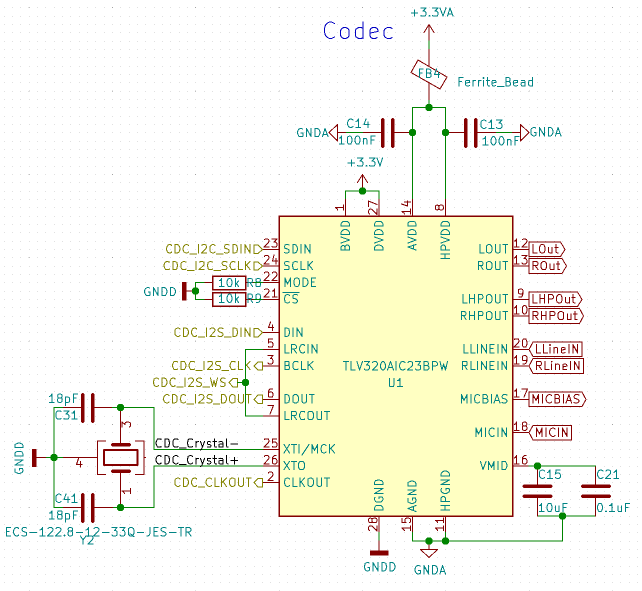
\includegraphics[scale=0.5]{../graphics/Schema_Codec.png}
\caption{TLV320AIC23B Codec von Texas Instruments}
\label{fig:Schema_Codec}
\end{center}
\end{figure}

Die Analog-Speisung des TLVs wird neben den 100\si{nF} Stütz-Kondensatoren zusätzlich von einem Ferrit Bead geglättet. Damit wird sichergestellt, dass keine ungewollten hochfrequente Spitzen in der Speisung das Audio-Signal verfälschen.

Intern sind die Audio-Eingänge des Codecs mit der halben Speisespannung (im Datenblatt VMID genannt) biased, sprich mit einem Offset versehen, damit nur positive Spannungen vorkommen.
In den nachfolgenden Unterkapiteln wird genauer auf die In- und Outputs des DSP-Boards, beziehungsweise deren äusseren Beschaltung eingegangen.


\paragraph{Line Input}
\label{par:LineIN}
Das Line-Signal wird am Eingang (Abbildung \ref{fig:Schema_LineIN}) erstmal durch den Spannungsteiler mit \textit{R23} und \textit{R14} bzw. \textit{R27} und \textit{R26} halbiert. Im Datenblatt des TLV320AIC23B \cite{tlv320} wird empfohlen die Signal-Amplitude von 2V auf 1V runterzubringen. Zudem bilden \textit{R23/R26} zusammen mit \textit{C23/C26}  einen Tiefpass-Filter mit einer Grenzfrequenz von 604.7 MHz (nach Gleichung \ref{eq:fg}), was schonmal die gröbsten hochfrequenten Störungen filtert. Mit \textit{C24/C20} wird das Signal zusätzlich galvanisch entkoppelt. Da der Audio-Eingang grundsätzlich eher hochohmig gehalten werden sollen, sind die Widerstands-Werte mit 5.6k$\Omega$ nicht zu klein gewählt. \cite{book:douglas}
Über den Tip-Switch des Mini-Jack-Steckers kann an einem GPIO-Pin des Microcontrollers auch detektiert werden ob ein Stecker eingesteckt ist, oder nicht.

\begin{equation}
f_g=\frac{1}{2\pi \cdot R \cdot C}
\label{eq:fg}
\end{equation}

\begin{figure} [H]
\begin{center}
 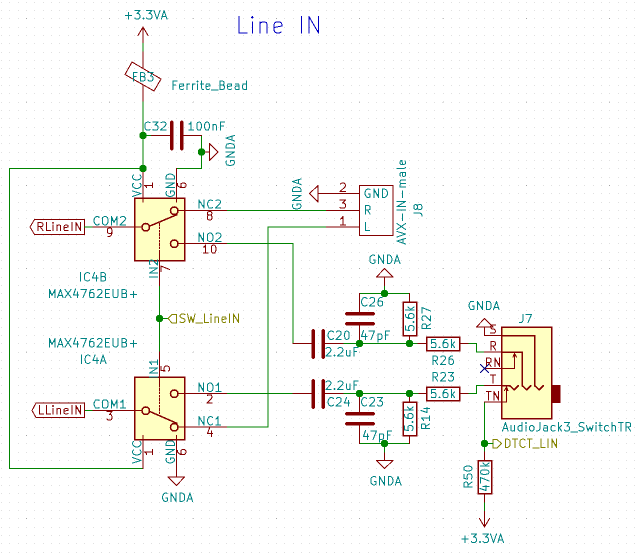
\includegraphics[scale=0.5]{../graphics/Schema_LineIN.png}
\caption{Schaltung Line Eingangsstufe mit Audio-Switch}
\label{fig:Schema_LineIN}
\end{center}
\end{figure}

Parallel dazu kommt über einen AVX-Stecker alternativ ein Audio-Signal von einem nächsten DSP-Board rein. Die Auswahl des Line-In Signals erfolgt über einen MAX4762 \cite{max4762} Audioswitch von Maxim der über einen GPIO-Pin des Microcontrollers angesteuert wird. 

\paragraph{Line Output}
\label{par:LineOUT}
An der Ausgangsstufe des Codecs wird mit einem Hochpass mit einer Grenzfrequenz von 1.54Hz (nach Gleichung \ref{eq:fg}), realisiert durch \textit{C7/C16} und \textit{R10/R11}, der DC-Anteil rausgefiltert um Brummen auf der Leitung zu verhindern.
Wie am Eingang wird hier der Ausgang parallel an einen AVX-Stecker geführt, um die Kaskadierung verschiedener Boards möglich zu machen.


\begin{figure} [H]
\begin{center}
 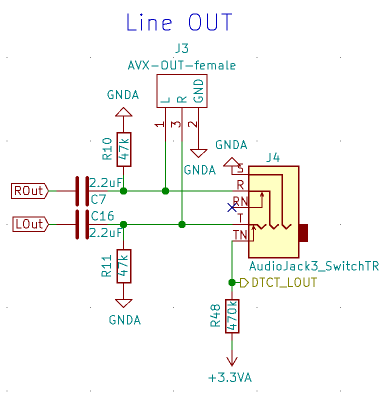
\includegraphics[scale=0.5]{../graphics/Schema_LineOUT.png}
\caption{Schaltung Line Ausgangsstufe}
\label{fig:Schema_LineOUT}
\end{center}
\end{figure}


\paragraph{Headphone Output}
\label{par:HPOUT}
Wie schon in der Line-Ausgangsstufe werden am Kopfhörer mit einem Hochpass, bestehend aus \textit{R4/R5} und \textit{C8/C9}, DC-Anteile rausgefiltert. Hier kommt parallel zu den Widerständen die Impedanz des Kopfhörers dazu (gängig sind $32\Omega$) was zu einer Grenzfrequenz von 22.61Hz führt (nach Gleichung \ref{eq:fg}). Durch die relativ kleine Impedanz des Kopfhörers müssen die Kondensatoren grösser sein um die Grenzfrequenz niedrig zu halten. Dies legt nahe polarisierte Elektrolytkondensatoren (sogenannte Elkos) zu verwenden, welche in Audio-Anwendungen oft zum Einsatz kommen.

\begin{figure} [H]
\begin{center}
 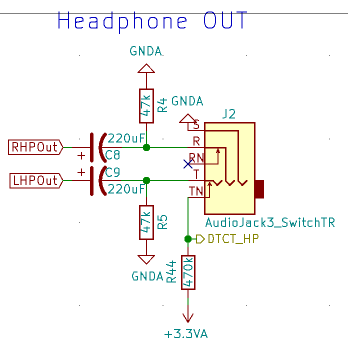
\includegraphics[scale=0.5]{../graphics/Schema_HPOUT.png}
 \caption{Schaltung Kopfhörer-Ausgang}
\label{fig:Schema_HPOUT}
\end{center}
\end{figure}


\paragraph{Mikrofon Input}
\label{par:MicIN}
Am Mikrofon-Eingang wird über den Seriewiderstand \textit{R3} der Eingangs-Gain des Codecs eingestellt. Laut Datenblatt des TLV320 \cite{tlv320} berechnet sich der Gain wie folgt:
\begin{equation}
A=\frac{50k\Omega}{10k\Omega+R_{Mic}}
\end{equation}
In der Schaltung \ref{fig:Schema_MicIN} entspricht $R_{Mic}$ \textit{R3} und ergibt somit einen Gain von -1.14dB (was nahezu eine Verstärkung von 1 macht).
Für Electret-Kondensator-Mikrofone hat der Codec einen MICBIAS-Pin, welcher das Mikrofon speist.
\begin{figure} [H]
\begin{center}
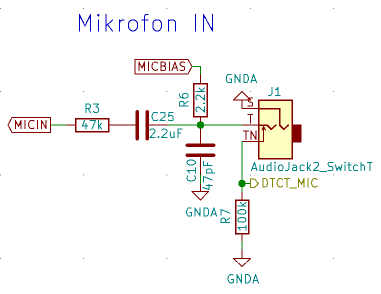
\includegraphics[scale=0.5]{../graphics/Schema_MicIN.png}
\caption{Schaltung des Mikrofon-Eingang}
\label{fig:Schema_MicIN}
\end{center}
\end{figure}

\paragraph{GND-Trennung}
Um zu verhindern, dass grössere rückfliessende Ströme im Digitalbereich Einfluss auf das Audio-Signal haben, wurden die GND-Planes für Analog- und Digital-Bereich grösstmöglich getrennt. Das ganze Board wurde in diese zwei Bereiche unterteilt und nur an einer Stelle mit \textit{R18} ($0\Omega$) verbunden. (Abbildung \ref{fig:Schema_GND})

\begin{figure} [H]
\begin{center}
 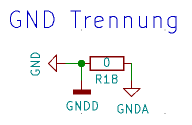
\includegraphics[scale=0.5]{../graphics/Schema_GND.png} 
\caption{Trennung der GND-Planes durch einen $0\Omega$ Widerstand}
\label{fig:Schema_GND}
\end{center}
\end{figure}



 